%% Introduction
\section{Methods}
%An overview of the physical components in the setup is shown in \autoref{fig:SystemOverview}.
\autoref{fig:SystemOverview} shows a head fitted with an ANC headphone using a reference microphone (1), a headphone loudspeaker (2), an error microphone (3) and a DSP (4).


%\begin{figure}[H]
%	\centering
%	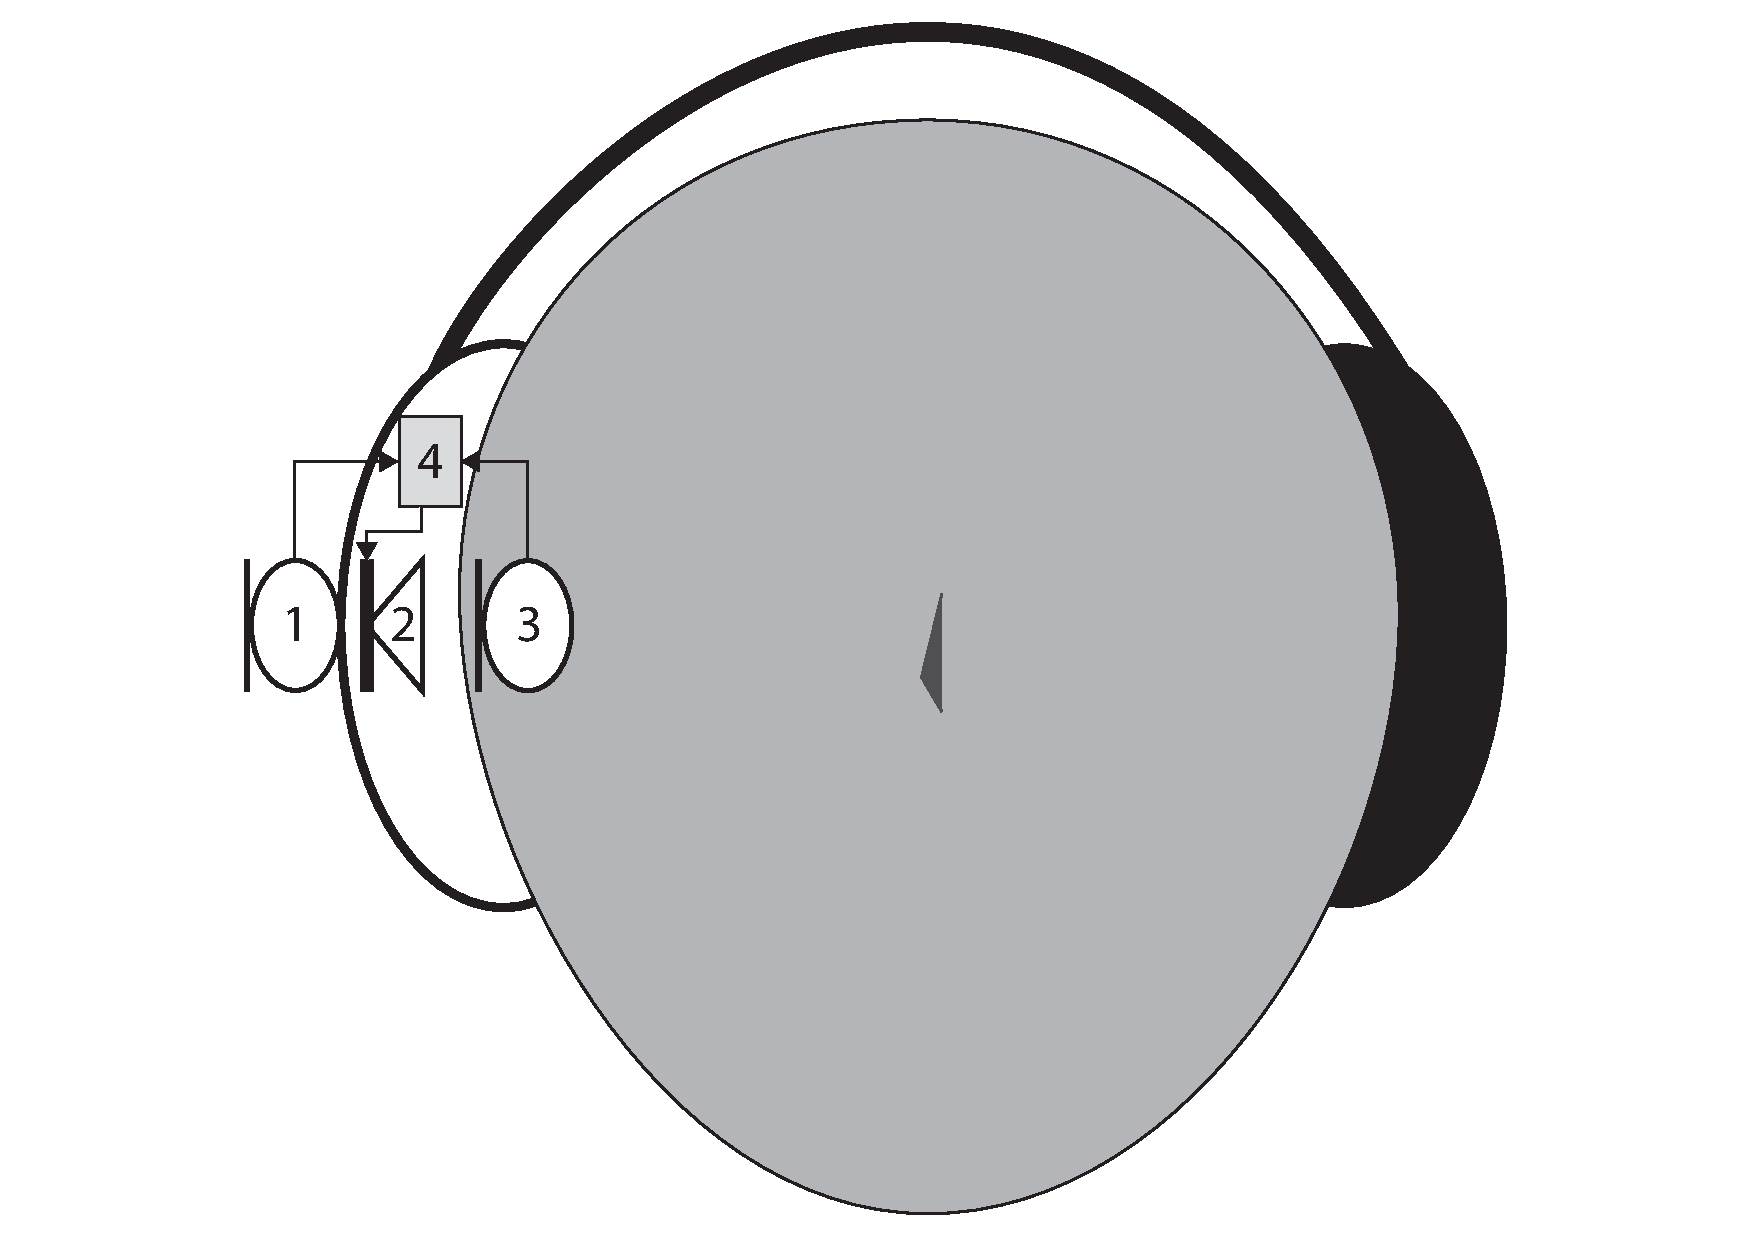
\includegraphics[width=1\columnwidth]{figures/ArticleIllustrations/SystemOverview}
%	\caption{System Overview}
%	\label{fig:SystemOverview}
%\end{figure}



\subsection{Feedforward ANC using FXLMS}
%The adaptive feedforward ANC system is shown on \autoref{fig:ANCFeedforward}
\autoref{fig:ANCFeedforward} shows an expansion of the DSP-block from \autoref{fig:SystemOverview}. This consists of converters and a control filter which is a FIR-filter where the coefficients are adapted by the FXLMS-algorithm. 
{
	%\centering
	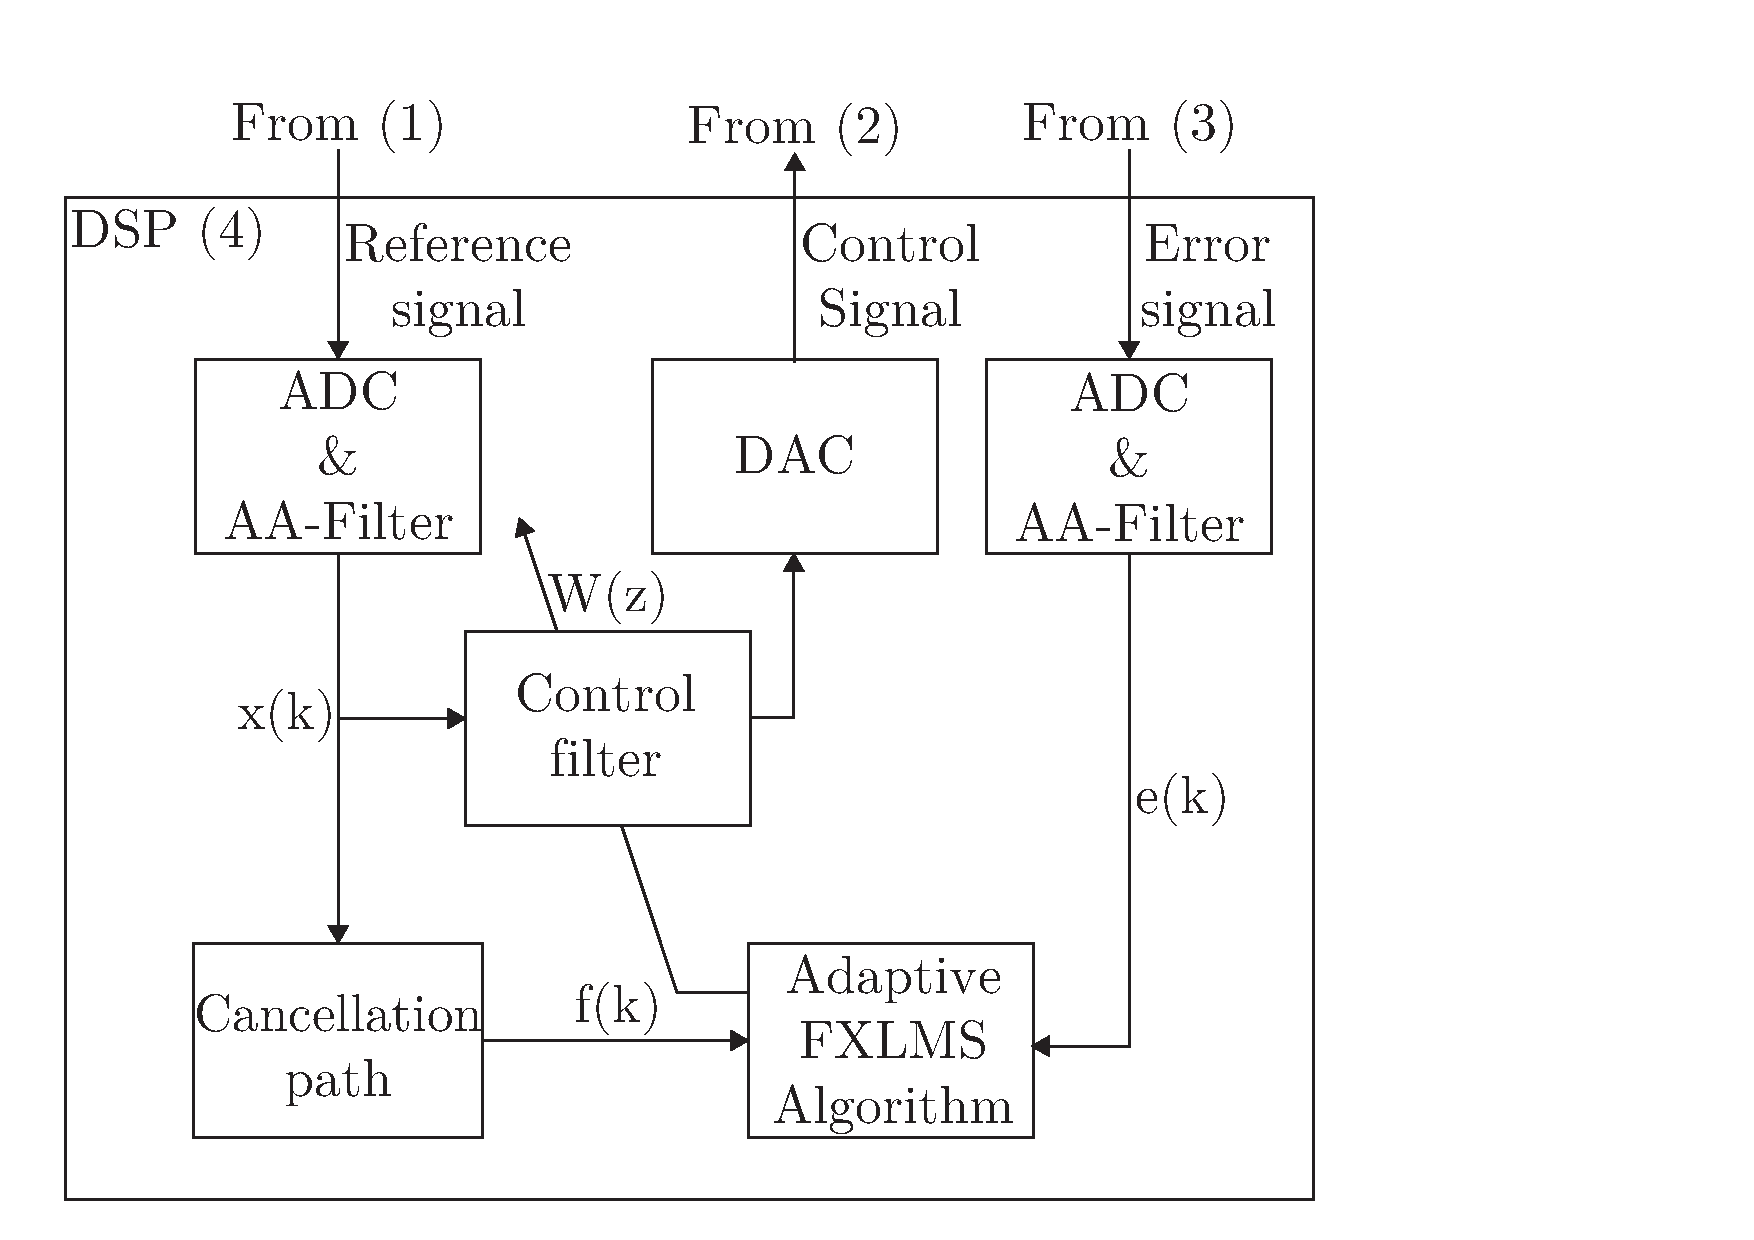
\includegraphics[width=1\columnwidth]{figures/ArticleIllustrations/ANCFeedForward}
	\captionof{figure}{Adaptive feedforward ANC system.}
	\label{fig:ANCFeedforward}
}

%\begin{figure}[H]
%	\centering
%	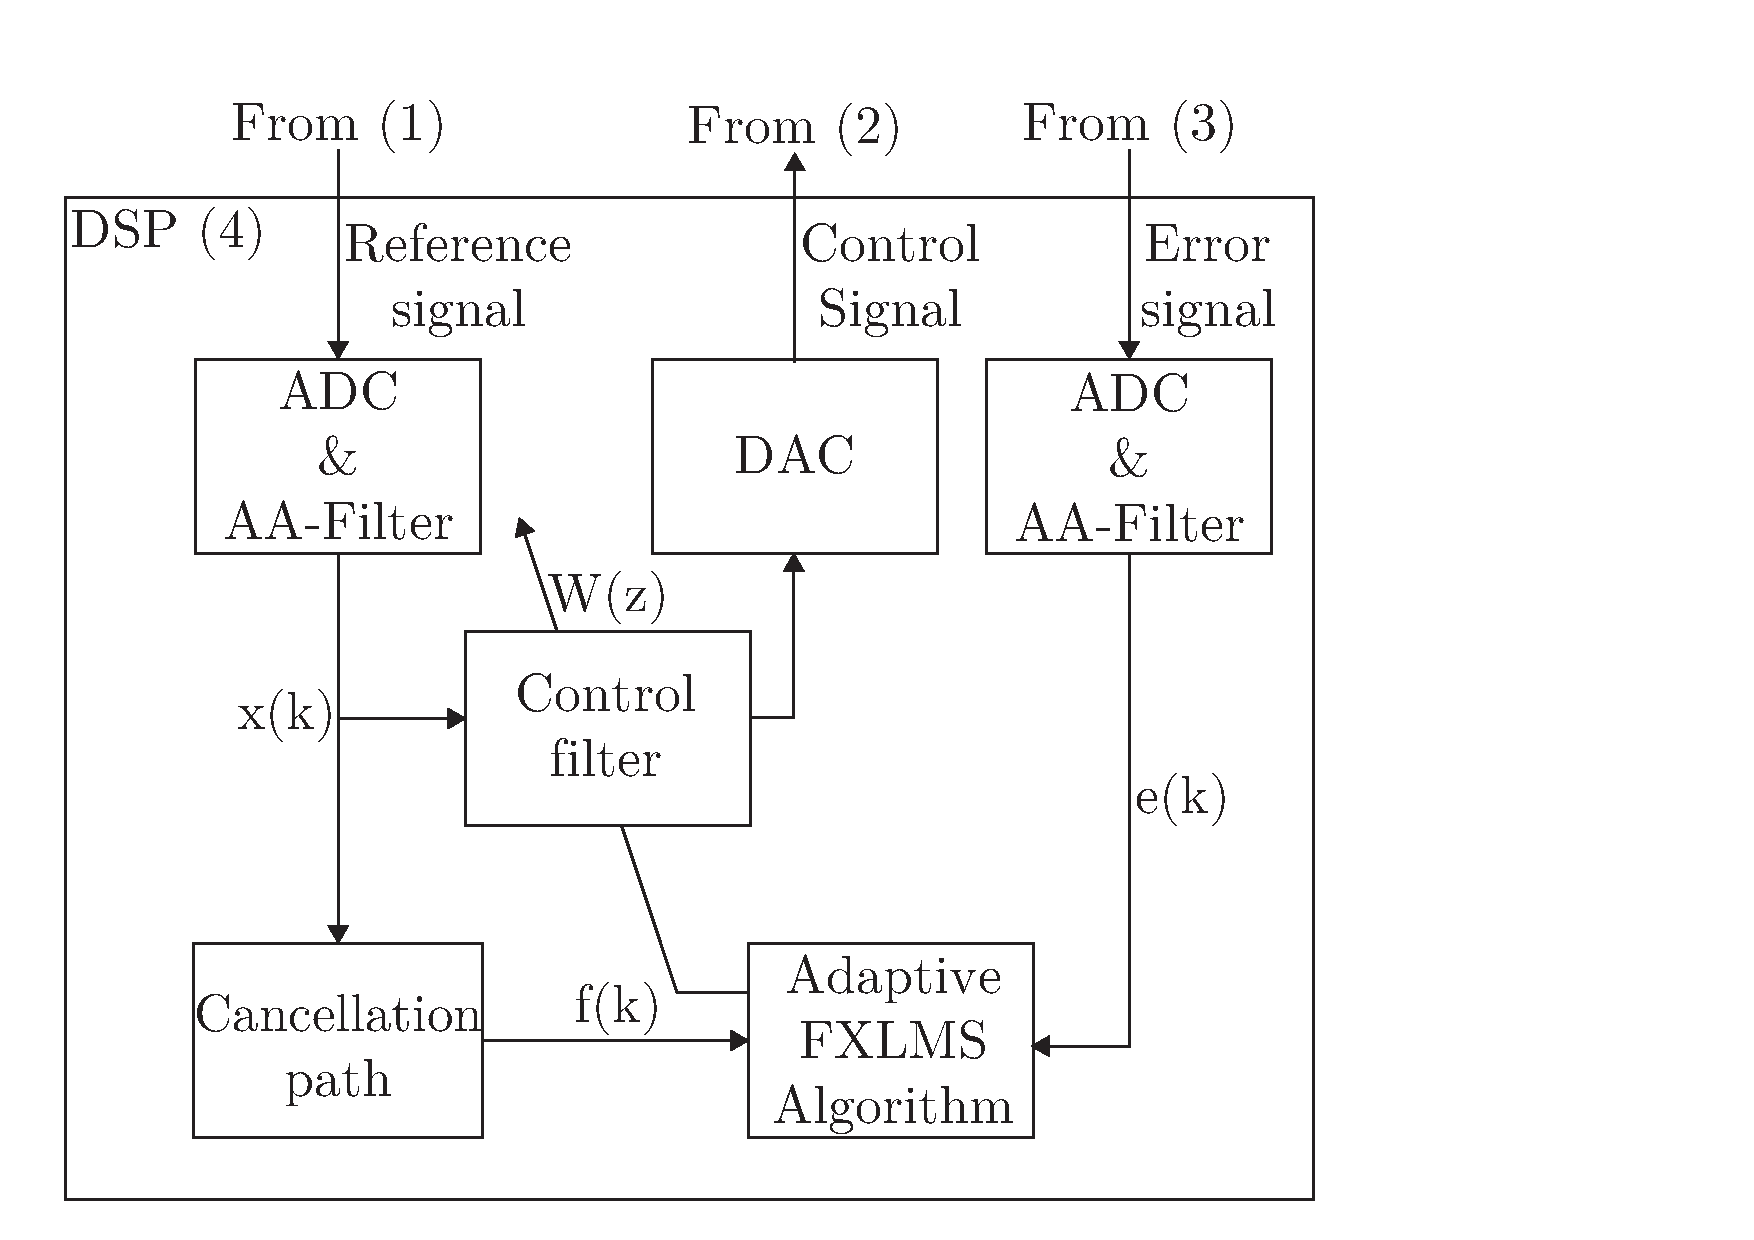
\includegraphics[width=1\columnwidth]{figures/ArticleIllustrations/ANCFeedForward}
%	\caption{Adaptive feedforward ANC system}
%	\label{fig:ANCFeedforward}
%\end{figure}


\textbf{Control Filter} is the filter representing the transfer function from the reference microphone to the headphone loudspeaker. The filter, shown in equation \ref{eq:Output}, is initialized with the inverse of the first 256 samples from the impulse response of the transfer function found by measurements in \autoref{sec:AngleOfIncidence}.  
\vspace{-3mm} % yeah I know - Sorry Mikkel!
\begin{equation}\label{eq:Output}
y[n]=\sum_{n=0}^{L-1}b_j[n]x[n-j]
\end{equation}
Where:
\vspace{-7mm} % yeah I know - Sorry Mikkel!
\begin{description}
	\item[\text{$b_j[n]$}] is the weight coefficients written as  $b[n]=[b_0[n],b_1[n], \cdots, b_{L-1}[n]]^T$
\end{description}

\textbf{FXLMS} is the optimization algorithm which updates the control filter coefficients using the FXLMS method shown in \autoref{eq:FXLMS} and derived in \autoref{sec:systemDesign}. 
\begin{equation}\label{eq:FXLMS}
b_j[n+1] = b_j[n] - 2\mu e[n]f[n-j]
\end{equation}
Where:
\vspace{-8mm} % yeah I know - Sorry Mikkel!
\begin{description}
	\item[\text{$\mu$}] is the convergence factor
	\item[\text{$e[n]$}] is the error 
	\item[\text{$f[n]$}] is the reference convolved with the Cancellation Path
\end{description}

\textbf{Cancellation Path} (CP) is the transfer-function from the headphone loudspeaker to the error microphone. In the literature \cite{Hansen} the CP is adaptively adjusted, but it is assumed constant in this setup because the headphone position is fixed.     


When implementing the system, delays exist due to the anti-aliasing and reconstruction filters. The delays of the system exceeds the propagation time of sound from the reference microphone to the headphone loudspeaker resulting in poor performance. Therefore an LP-algorithm is proposed to predict future samples in order to decrease the effect of the time delays.

\subsection{Characteristic of Speech}
Speech can be split into two main classes, voiced and unvoiced. Voiced sounds are characterized by a strong periodicity, with the fundamental frequency referred to as the pitch frequency (50 - 500 Hz). Unvoiced sounds are characterized as random. Speech is a non stationary signal and can only be assumed wide sense stationary (WSS) for periods of 20 - 30 ms\cite{SpeechCharacteristics}. 

\subsection{Linear Prediction of Speech}
In order to predict future samples the auto correlation function (ACF), which is used in LP, of speech must be estimated in frames. The outlines of the prediction system is shown in figure \ref{fig:LinearPredictionOverview}.

\begin{figure}[H]
	\centering
	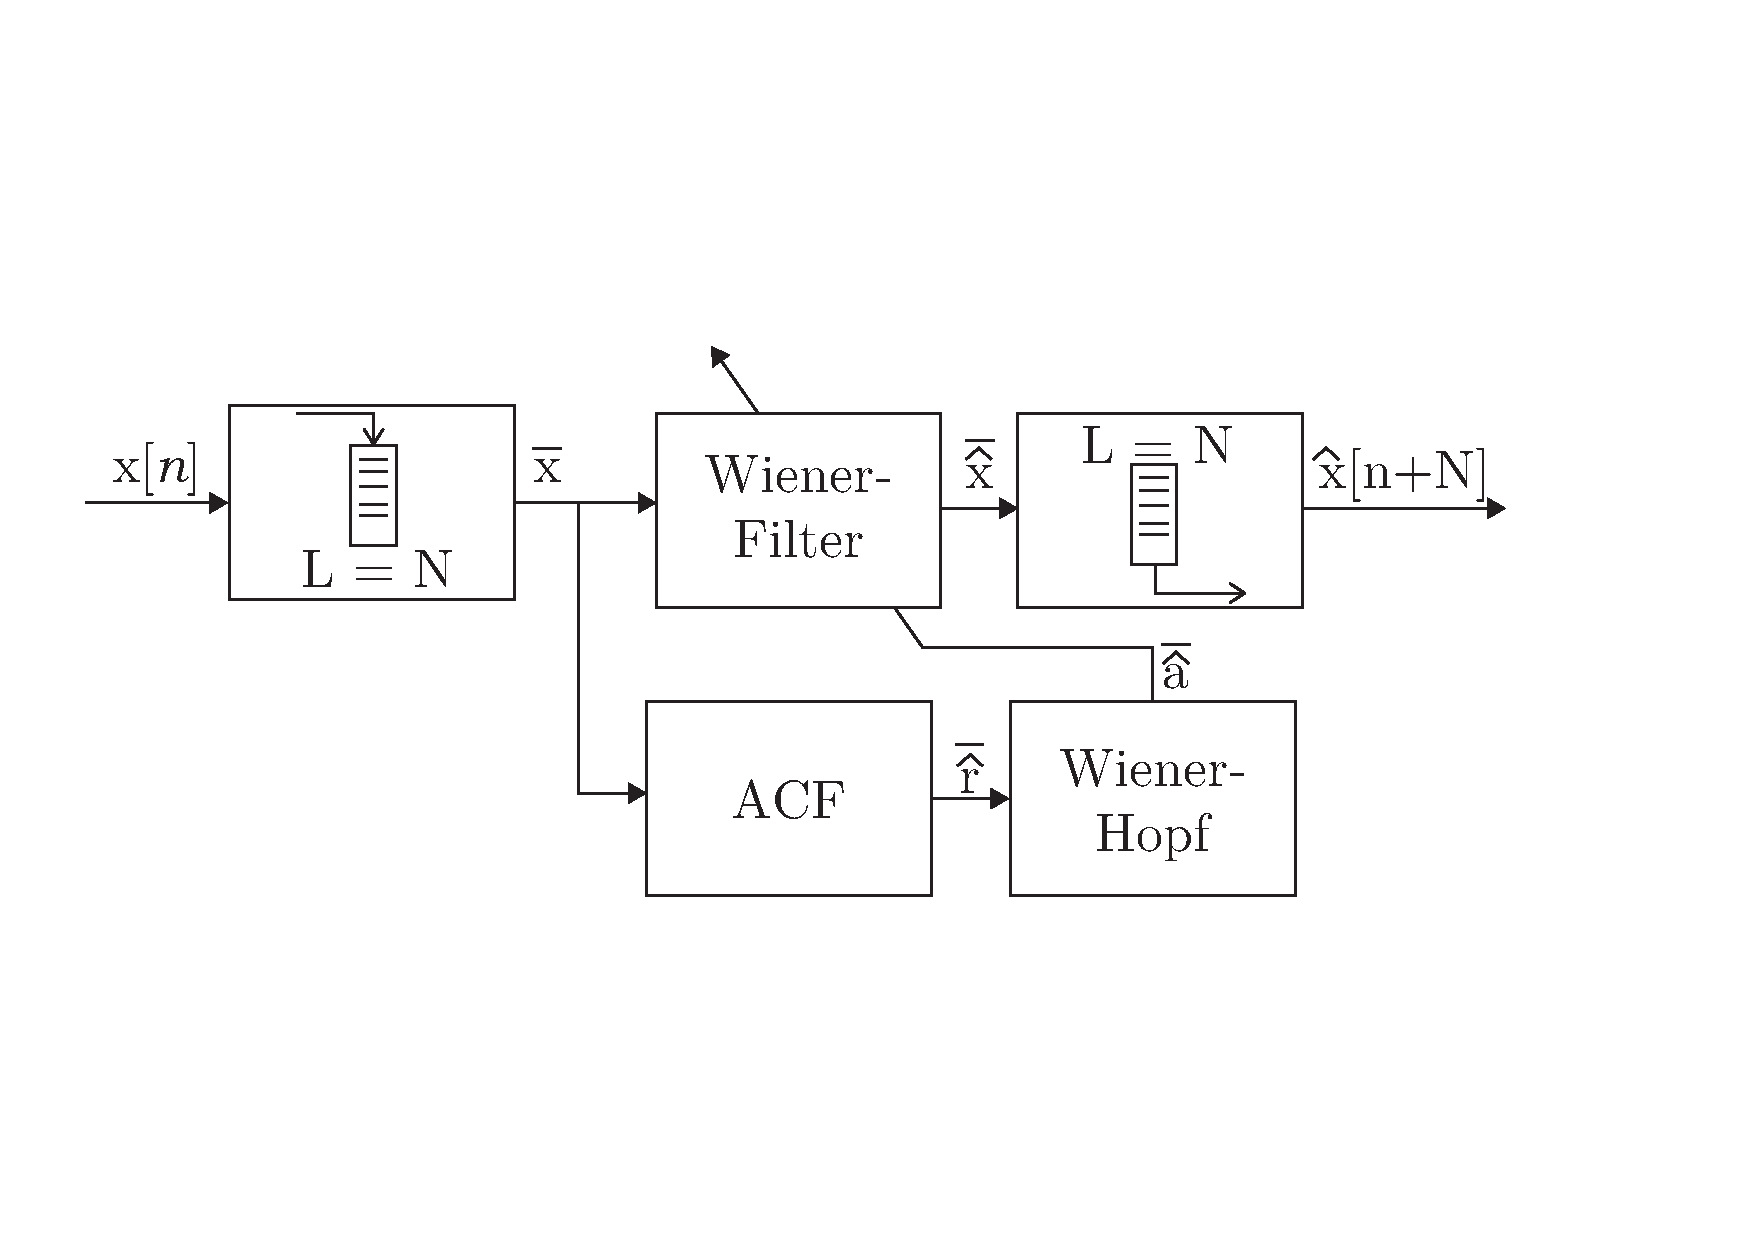
\includegraphics[width=\columnwidth]{ArticleIllustrations/WienerHopf}
	\caption{Linear prediction overview}
	\label{fig:LinearPredictionOverview}
\end{figure}


Utilizing a nonrecursive estimation of the ACF, shown in \autoref{eq:nonrecursive}, it is possible to determine the linear prediction coefficients (LPCs) which are used for predicting future samples \cite{LinearPrediction}. When estimating the ACF of the input ($x$) a Hamming window ($w$) is applied.
\begin{equation}\label{eq:nonrecursive}
%%r_x[l,m] = \sum^{m}_{n=m-N+1+\left| l\right|} x_l[n]w_l[m-n]
r_x[l] = \sum^{N}_{n=\left| l\right|} x_l[n]w_l[N-n]
\end{equation}
%\begin{multline}\label{eq:nonrecursive}
%R[l,m] = \sum^{m}_{n=m-N+1+\left| l\right|} \\ x[n]w[m-n] x[n-\left| l\right|]w[m-n+\left| l\right|]
%\end{multline}
%\begin{equation}
%R[l,m]=\sum^{m}_{n=m-N+1+\left| l\right|}x[n]w[m-n] x[n-\left| l\right|]w[m-n+\left| l\right|]
%\end{equation}
Where:
\vspace{-8mm}
\begin{description}
	\item[\text{$x_l[n]$}] $=x[n]x[n-l]$ 
	\item[\text{$w_l[n]$}] $=w[n]w[n+l]$
	\item[\text{$l$}] is the lag 
	\item[\text{$m$}] is the frame index
	\item[\text{$N$}] is the frame size
\end{description}
The LPCs are determined using \autoref{eq:normal}, known as the Wiener-Hopf equation.
\begin{equation}\label{eq:normal}
R \cdot \bar{a} = -\bar{r_x}
\end{equation}
Where:
\vspace{-8mm} % yeah I know - Sorry Mikkel - again!
\begin{description}
	\item[\text{$R$}] is the covariance matrix $C_{xx}$
	\item[\text{$\bar{a}$}] is the LPCs, $\bar{a} = [a_1 , a_2, \cdots, a_N]^T$
	\item[\text{$\bar{r_x}$}] is the ACF, $\bar{r_x} = [r_x[1] , r_x[2], \cdots, r_x[N]]^T$
\end{description}
\autoref{eq:normal} can be rewritten as shown in \autoref{eq:normal2} yielding the LPCs directly.  
 \begin{equation}\label{eq:normal2}
\bar{a} = -R^{-1}\cdot \bar{r_x}
\end{equation}
Calculating $R^{-1}$ is computationally heavy on a DSP. To estimate the LPCs the Levinson-Durbin method is used. Prediction using wiener filtering, shown in equation \ref{eq:Predictor}, can then be applied to the current frame for prediction of the next frame. 

\begin{equation}\label{eq:Predictor}
\hat{x}[n+1] =- \sum^{N}_{i=1}a_ix[n-i]
\end{equation}

Using equation \ref{eq:Predictor} in cascade where $\hat{x}[n+2]$ is estimated using $\hat{x}[n+1]$ and $x[n]$. The predicted frame is then used as input for the ANC system.

